\documentclass[12pt]{article}
\usepackage{float}
\usepackage{sbc-template}
\usepackage{graphicx,url}
\usepackage[brazil]{babel}   
\usepackage[utf8]{inputenc}  
\usepackage{indentfirst}
\usepackage{caption3}
\usepackage{color}
\usepackage{alltt}
\usepackage{url}
\usepackage{listings}

\lstset{ %
language=C,                % choose the language of the code
basicstyle=\footnotesize,       % the size of the fonts that are used for the code
numbers=left,                   % where to put the line-numbers
numberstyle=\footnotesize,      % the size of the fonts that are used for the line-numbers
stepnumber=1,                   % the step between two line-numbers. If it is 1 each line will be numbered
numbersep=7pt,                  % how far the line-numbers are from the code
backgroundcolor=\color{white},  % choose the background color. You must add \usepackage{color}
showspaces=false,               % show spaces adding particular underscores
showstringspaces=false,         % underline spaces within strings
showtabs=false,                 % show tabs within strings adding particular underscores
frame=single,           % adds a frame around the code
tabsize=2,          % sets default tabsize to 2 spaces
breaklines=true,        % sets automatic line breaking
breakatwhitespace=false,    % sets if automatic breaks should only happen at whitespace
escapeinside={\%*}{*)},          % if you want to add a comment within your code
extendedchars=true,
emph={%  
    set, pair, bool%
    },emphstyle={\bfseries},
morekeywords={set, pair}
literate={á}{{\'a}}1 {ã}{{\~a}}1 {é}{{\'e}}1
}
     
\sloppy

\title{siC: Uma linguagem baseada em C incluindo pilha, lista e fila como tipos primitivos}

\author{Gabriella de Oliveira Esteves, 110118995}

\address{Departamento de Ciência da Computação - Universidade de Brasília}

\begin{document} 

\maketitle

%------------------------------------------------
\section{Objetivo}

Este trabalho visa projetar e construir uma nova linguagem chamada de siC - Structures in C, baseada na linguagem C. O siC acrescenta três estruturas de dados, lista, pilha e fila, como tipos de dados primitivos e, para manipulá-las, adiciona certas operações próprias para tal.

%------------------------------------------------
\section{Introdução}

\indent Um compilador é um programa que recebe como entraga um código fonte e o traduz para um programa equilavente em outra linguagem \cite{book}. Ele pode ser dividido em sete fases, ilustrado na Figura \ref{fig:compilador}.

\begin{figure}[!ht]
  \centering
  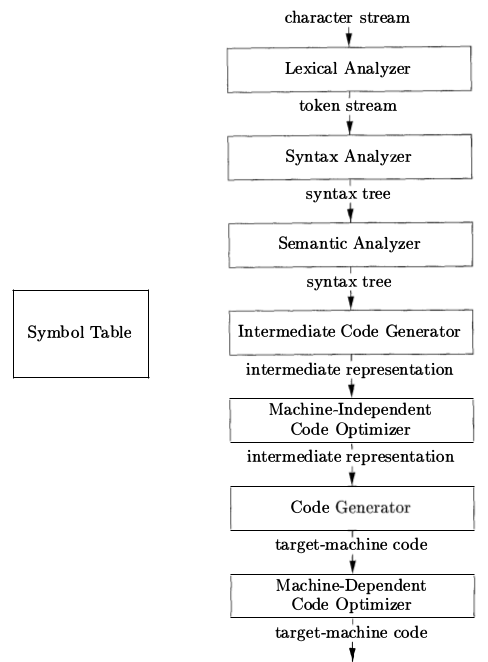
\includegraphics[width=0.5\textwidth]{compilador.png}
  \caption{Fases de um compilador} \label{fig:compilador}
\end{figure}

\begin{itemize}
	\item[1] \textbf{Analisador Léxico:} Lê o código fonte e atribui significado à cada sequência de caracteres, agora chamados lexemas. Cada lexema é mapeado para um token, que por sua vez é um par de nome (símbolo abstrato) e atributo (ponteiro para tabela de símbolos);
	\item[2] \textbf{Analisador Sintático:} Constrói uma representação gramátical dos tokens em forma de árvore;
	\item[3] \textbf{Analisador Semântico:} Utiliza a árvore sintática juntamente com a tabela de símbolos para verificar se a consistência semântica é mantida de acordo com a definição da linguagem.
	\item[4] \textbf{Gerador de Código Intermediário:} Converte árvore sintática anotada em código intermediário, com linguagem parecida com assembly e que possui apenas três operadores por linha de código. Nesse sentido, quebra-se estruturas complexas em estruturas mais simples, nesta fase.
	\item[5, 6] \textbf{Otimizador de Código Independente/Dependente de Máquina:} Procura aprimorar o código intermediário com o objetivo de melhorar o código-alvo de alguma forma: o deixando mais rápido, mais curto, consumindo menos energia, etc.
	\item[7] \textbf{Gerador de Código:} Converte o código intermediário no código-alvo, 	buscando atribuir os registradores às variáveis da maneira ótima.
\end{itemize}

\indent O foco do projeto será nas fase 1, 2, 3 e 4, porém a princípio serão apresentadas apenas a descrição da linguagem siC, bem como uma breve descrição de sua semântica.

\indent Dois grandes motivos sustentam a escolha do tema deste projeto. Primeiro, uma vez que as estruturas de dados pilha, fila e lista fazem parte dos tipos primitivos de uma linguagem, haverá menos manipulação de ponteiros na mesma, portanto erros envolvendo-os são menos prováveis de ocorrer. Segundo, a linguagem siC é mais alto-nível que C devido à abstração das estruturas de dados báscias, e, de maneira geral, pode ser mais \textit{user-friendly}. Nesse sentido, o usuário (da linguagem) leigo deverá entender como cada estrutura funciona, bem como suas vantagens/desvantagens e usabilidade; porém a implementação de cada uma estará a cargo da própria siC.


\section{Gramática}

\indent A seguir será apresentada a gramática da linguagem siC, que é unicamente baseada em C \cite{yacc}.

\vspace{2mm}
\begin{alltt}


basic\_expression
    : while\_expression
    | if\_expression
    | add\_expression
    | subtract\_expression
    | multiply\_expression
    ;
		
		
while\_expression
    :
    |
    ;


if\_expression
    :
    |
    ;
    
    
add\_expression
    :
    |
    ;
    
    
subtract\_expression
    :
    |
    ;
    
    
multiply\_expression
    :
    |
    ;
    
        
assignment\_operator	
    : '='
    | '+='
    | '-='
    | '*='
    ;
			
\end{alltt}
\vspace{2mm}

%\section{Analisador Léxico}

%\section{Analisador Sintático}

%\subsection{Árvore sintática}

%\subsection{Tabela de símbolos}

%\section{Analisador Semântico}

%\section{Geração de código intermediário}

% \section{Considerações finais}

\begin{thebibliography}{1}
\bibitem{book}
A.~V.~Abo, M.~S.~Lam, R.~Sethi, J.~D.~Ullman, \emph{Compilers - Principles, Techniques and Tools}
\hskip 1em plus
	0.5em minus 0.4em\relax 2nd ed. 1986
	
\bibitem{yacc}
ANSI C Yacc grammar, \url{http://www.quut.com/c/ANSI-C-grammar-y.html}, 18 12 2012.
\end{thebibliography}
%------------------------------------------------
\end{document}